% !TeX spellcheck = en_GB
\documentclass[10pt,letterpaper,oneside]{article}
\usepackage{fontspec}
\usepackage{arev}
\usepackage[utf8]{inputenc}
\usepackage[T1]{fontenc}
\usepackage{amsmath}
\usepackage{amsfonts}
\usepackage{amssymb}
\usepackage{graphicx}
\usepackage{csquotes}
\usepackage{booktabs}
\usepackage{multicol}
\usepackage{enumerate}
\usepackage{microtype}
\usepackage[labelfont=bf,font={small}]{caption}
\usepackage{hyperref}
\usepackage{booktabs}
\usepackage{subcaption}
\usepackage{fancyhdr}
\usepackage[svgnames]{xcolor}
\usepackage{mdframed}
\usepackage{multicol}
\usepackage[para]{footmisc}
\usepackage{siunitx}
\usepackage{cleveref}
\usepackage{listings}
\usepackage{cprotect}


\lstset{ % General setup for the package
	language=Python,
	basicstyle=\small\ttfamily,
	tabsize=4,
	columns=fixed,
	showstringspaces=false,
	showtabs=false,
	keepspaces,
	commentstyle=\color{SeaGreen},
	keywordstyle=\bf\ttfamily\color{DarkBlue},
	stringstyle=\ttfamily\color{Crimson}
}

\newfontfamily\symbolfont{Symbola}
\usepackage[left=1in,right=1in,top=1in,bottom=1in,marginparwidth=0.3in]{geometry}

\usepackage[sorting=none]{biblatex}
\addbibresource{../bibliography.bib}

\ifx\NoteAuthor\undefined
  \def\NoteAuthor{Andreas Stöckel and Chris Eliasmith}
\fi

\ifx\BasedOn\undefined
  \def\BasedOn{Based on lecture notes by\\Chris Eliasmith and Terrence~C.~Stewart}
\fi

\author{\NoteAuthor\\[0.5cm]\BasedOn}
\newcommand{\baseCodeURL}{https://github.com/celiasmith/syde556-f23/blob/master/lectures}

\fancyhf{}
\fancyhead[L]{SYDE 556/750 Lecture Notes}
\fancyhead[R]{\NoteAuthor}
\fancyfoot[C]{\thepage}
\pagestyle{fancy}

\setlength{\parindent}{0em}
\setlength{\parskip}{0.5em}
\renewcommand{\baselinestretch}{1.25}

\renewcommand{\vec}[1]{{\mathbf{#1}}}
\newcommand{\mat}[1]{{\mathbf{#1}}}
\newcommand{\T}{\ensuremath{\mathrm{T}}}
\renewcommand{\epsilon}{\varepsilon}
\renewcommand{\phi}{\varphi}

\makeatletter
\newcommand{\superimpose}[2]{%
	{\ooalign{{#1}\hidewidth\cr{#2}\hidewidth\cr}}}
\makeatother
\newcommand{\SolidCircle}[2]{\superimpose{\color{#1}\symbolfont ⬤}{\textbf{\color{white}#2}}\hspace{1em}}
\newcommand{\OPlus}{\SolidCircle{DarkGreen}{\kern0.75pt+}}
\newcommand{\OMeh}{\SolidCircle{DarkOrange}{~}}
\newcommand{\OMinus}{\SolidCircle{DarkRed}{\kern2.25pt--}}

\newcommand{\YouTube}[2][Video]{\href{https://youtu.be/#2}{{\symbolfont 📺}~{#1}}%
%\footnote{\url{https://youtu.be/#2}}%
}

\newcommand{\CodeLink}[2][Code]{\href{\baseCodeURL/#2}{{\symbolfont ⌨}~\emph{#1}}}

\newcommand{\MakeTitle}[1]{
\maketitle
\begin{center}
	
\includegraphics[width=0.5\textwidth]{../assets/uwlogo.pdf}\\[1cm]
	{#1}\
\end{center}

\vfill

\thispagestyle{empty}
\setcounter{page}{0}
\newpage

\pagenumbering{roman}
\setcounter{tocdepth}{2}
\tableofcontents
\newpage

\setcounter{page}{0}
\pagenumbering{arabic}}

\reversemarginpar


\newcommand{\ColorBox}[3]{%
	\marginpar{%
		\huge\raisebox{-3ex}{\symbolfont{#1}}%
	}%
	\begin{mdframed}[hidealllines=true,backgroundcolor=#2,innertopmargin=0.25cm,innerbottommargin=0.25cm]%
		{#3}
	\end{mdframed}}

\newcommand{\Note}[1]{\ColorBox{📌}{WhiteSmoke}{\textbf{Note:} #1}}
\newcommand{\Example}[1]{\ColorBox{💡}{WhiteSmoke}{\textbf{Example:} #1}}
\newcommand{\Aside}[1]{\ColorBox{🌟}{WhiteSmoke}{\emph{Aside:} #1}}
\newcommand{\Python}[1]{\ColorBox{🐍}{WhiteSmoke}{#1}}
\newcommand{\Notation}[1]{\ColorBox{\huge$\Sigma$}{WhiteSmoke}{\textbf{Notaton:} #1}}

\newcommand{\ConstructionSite}{\hrulefill {\symbolfont 🚧} UNDER CONSTRUCTION {\symbolfont 🚧} \hrulefill}

\newenvironment{ImportantEqn}[1]{\mdframed\raggedleft\emph{({#1})}\align}{\endalign\endmdframed}

\date{September 21, 2022}
\title{SYDE 556/750 \\ Simulating Neurobiological Systems \\ Lecture 7: Temporal Basis Functions}


\begin{document}

\MakeTitle{\textbf{Accompanying Readings: Chapter 3 of Neural Engineering; see references}}

\section{Introduction}

\begin{figure}[h]
	\centering
	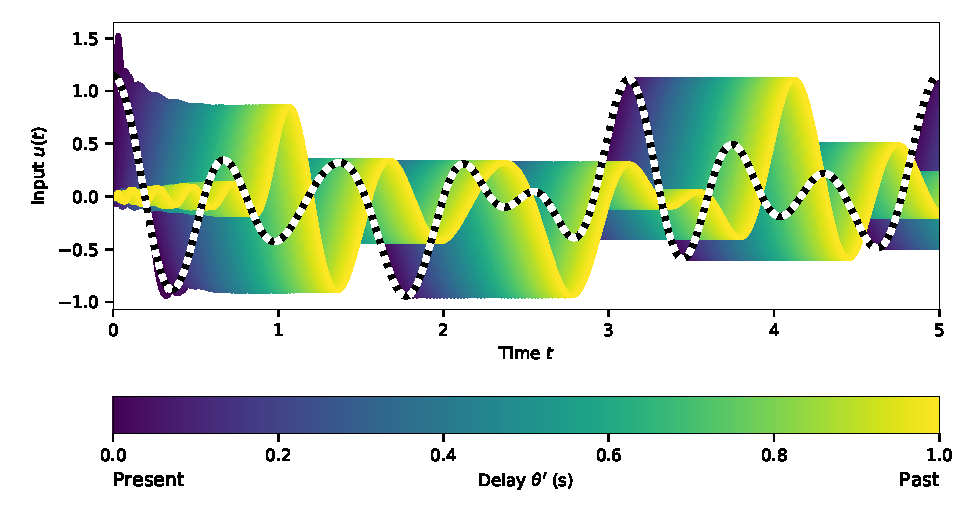
\includegraphics{media/delay_network_decoding.pdf}
	\caption{Example of the \enquote{delay network} we are going to discuss in the lecture. The dotted line is the input $u(t)$. The coloured lines correspond to delayed versions of the input signal. These delayed versions are all decoded from the same function representation $f_{[t - \theta, t]}(\theta')$. This diagram has been generated by decoding from a mathematically perfect implementation of the delay network. \CodeLink{lecture_07/media/code/delay_network_example.ipynb}}
\end{figure}

\Note{In this lecture we discuss a recent application of the Neural Engineering Framework, the so called Delay Network developed by Aaron Voelker, first presented in \cite{voelker2018improving}, and discussed in more detail in his PhD thesis \cite{voelker2019thesis}. The Delay Network represents a function over time in a neural population. A more general version of the Delay Network has been presented at NeurIPS 2019 as the \enquote{Legendre Memory Unit}~(LMU)~\cite{voelker2019lmu}. The LMU can be used as a component within artificial Deep Neural Networks and outperforms other recurrent architectures such as LSTMs in a variety of tasks.}

As humans, we often feel as if we have a good recollection of events that happened in the immediate past, where in this lecture, \enquote{immediate} refers to events happening within a few seconds or even a fraction of a second. As events move into the more distant past, it becomes increasingly harder to recall details. In this lecture, we discuss a system that similarly memorizes stimuli, remembers them for a certain period, and then gradually \enquote{forgets} them.

Mathematically speaking, what we would like to have a function $f_{[t - \theta, t]}(\theta')$ which allows us to access stimuli $u(t)$ in a time-interval from $[t - \theta, t]$, that is
\begin{align*}
	f_{[t - \theta, t]}(\theta') = u\left(t - \theta' \right) \,, \text{where } 0 \leq \theta' \leq \theta \,.
\end{align*}
Put differently, $f_{[t - \theta, t]}(0)$ will return the present stimulus $u(t)$, whereas $f_{[t - \theta, t]}(\theta)$ will return the input $\theta$ seconds from the past.

We would like to build a biologically plausible version of such a system. That is, we would like to represent information about the immediate past in the current activity of a population of neurons $f_{[t - \theta, t]}$. In order to do this, we have to solve two problems that we discuss separately.
\begin{enumerate}[1.]
	\item \textbf{Function representation.} So far we have seen how we can represent vectorial quantities in a neural population. But how can we represent an entire \emph{function} of the form $f_{[t - \theta, t]}(\theta')$ in a neural ensemble?
	\item \textbf{Updating the function representation.} If we were somehow able to represent functions in our neural population we still need to know how exactly to update this representation over time.
\end{enumerate}


\Note{Function \emph{representation} is different from the \enquote{transformation} principle we already discussed. In short, we are not interested in computing a function $\vec y = f(\vec x)$, but instead we would like to \emph{represent} the function $f$ itself in a neural population, i.e.~have some way of storing a mapping from a value $\vec x$ onto values $\vec y$.}

\section{Representing Functions}

For simplicity, and because it describes the problem we are trying to solve, let's focus on scalar functions over time $f(t)$, i.e., $f : \mathbb{R} \longrightarrow \mathbb{R}$. How can we represent an interval $[0, T)$ of such a function in a neural population? We already know how a neural population can represent a vector, so let's rephrase the question. How can we represent functions as vectors?

First of all, if we have a parametrised function family $f(t; \vec x)$ we want to represent (i.e., all linear functions, all affine functions, all Normal distributions with a mean $\mu$ and standard-deviation $\sigma$), then the function parameters can be described as a vector $\vec x$ that we could use:
\begin{align*}
	f(t; \vec x) &= m t \,, & \text{Linear function } &\Rightarrow \vec x = \begin{pmatrix}m\end{pmatrix} \,, \\
	f(t; \vec x) &= m t + b \,, & \text{Affine function } &\Rightarrow \vec x =  \begin{pmatrix}m, b\end{pmatrix} \,, \\
	f(t; \vec x) &= \exp\left(-\frac{(t - \mu)^2}{\sigma^2}\right) \,,  & \text{Gaussian } &\Rightarrow \vec x =  \begin{pmatrix}\mu, \sigma\end{pmatrix} \,.
\end{align*}
If we represent $\vec x$ and $t$ in the same neural population, we can evaluate $f(t; \vec x)$ in the connection from the pre- to the post-population according to NEF principle two.

In general, if we do not have any more information about the kind of function we would like to represent, there are two (closely related) approaches to representing functions as vectors: sampling/discretisation and basis functions. We discuss these two approaches in the following.

\Note{We can generalise what we discuss to multi-variate functions with vectorial output, i.e. $f : \mathbb{R}^d \longrightarrow \mathbb{R}^{d'}$. We can treat multi-dimensional \emph{output} $d' > 1$ as $d'$ independent functions $f_1, \ldots, f_{d'}$. For multi-dimensional \emph{inputs} $d > 1$, we need to sample on a higher-dimensional grid. When using basis functions, we need an appropriate basis $\phi_i : \mathbb{R}^{d} \longrightarrow \mathbb{R}$.}

\subsection{Sampling}

The idea of sampling is to measure the value of a function $f(t)$ at discrete, equally spaced points $\vec x = ( x_0, \ldots, x_{N - 1} )$, where
\begin{align*}
	x_i &= f(t_i) = f(\Delta t i) \,, & \text{and } \Delta t \text{ is the sampling interval.}
\end{align*}
The resulting vector $\vec x$ holds a representation of $f(t)$ over the interval $[0, T)$, where $T = N \Delta t$.

If we wanted the reconstruct the value of the function at a point $t$ that was not sampled, we can in theory use one of many interpolation techniques to \enquote{guess} function values in between samples. If our function is somewhat well-behaved, we would expect the quality of these reconstructions to get better for smaller $\Delta t$. That is, the more sample points $N$ we have over the interval $[0, T)$, the better the representation of the function (\cref{fig:sampling}).

Unfortunately, in general, for an arbitrary function $f(t)$, we need an infinite number of sample points to perfectly represent it. Mathematically speaking this is true for any infinitesimally small interval $T \to 0$. A function can \enquote{drastically} change its value between any two infinitesimally close points.

\Example{These restrictions even apply to continuous functions! The earliest example of a \enquote{weird} continuous function that is not differentiable (i.e., not \enquote{smooth}) at any point is the Weierstrass function published in 1872, defined as
\begin{align*}
	f(x) &= \sum_{n = 0}^\infty a^n \cos(\pi b^n x) \,, & \text{where } 0 < a < 1, b \text{ is a positive odd integer, and } ab > 1 + \frac{3}2 \pi \,.
\end{align*}
Intuitively, this function is continuous at any point---after all, it is just a sum of cosines (be careful though; counter-intuitively, an \emph{infinite} sum of continuous functions \emph{can} be discontinuous). One can show that this function is not differentiable at any point. %(the infinite series diverges independent of $x$ for the derivative).

{\centering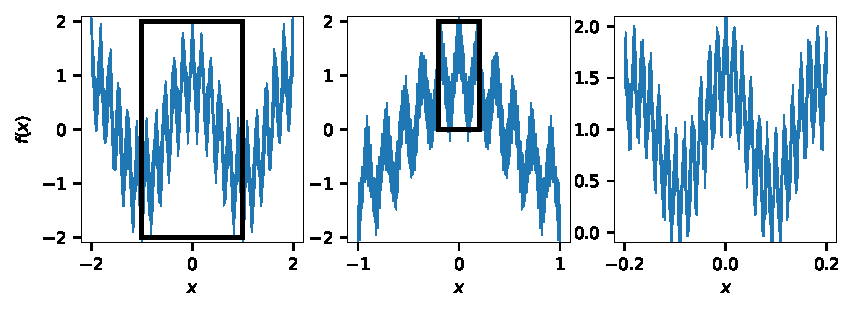
\includegraphics{media/weierstrass.pdf}\\}
{\small\addtocounter{figure}{1}\textbf{Figure \arabic{figure}.} Visualisation of the Weierstrass function for $b = 11$, $a =  \frac{1 + \frac{3}2 \pi}{10}$. Black rectangles correspond to the region shown in the neighbouring plot to the right. No matter how far we \enquote{zoom} into the function, there is an infinite amount of detail we would have to capture when sampling (this is one of the properties of a \emph{fractal}; note that this does not necessarily imply an infinite amount of \emph{information} in this function; the function is fully determined by two parameters $a$, $b$). \CodeLink{lecture_07/media/code/weierstrass.ipynb}}}


\begin{figure}
	\begin{subfigure}{\textwidth}
		\centering
		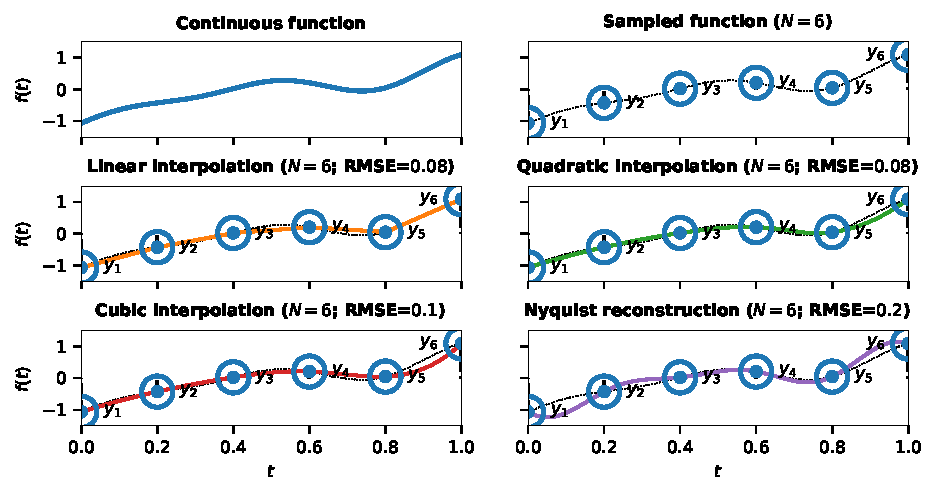
\includegraphics{media/fun_1_q6_small.pdf}
		\caption{Example 1: Bandlimit above $\SI{3}{\hertz}$}
	\end{subfigure}\\[0.5cm]
	\begin{subfigure}{\textwidth}
		\centering
		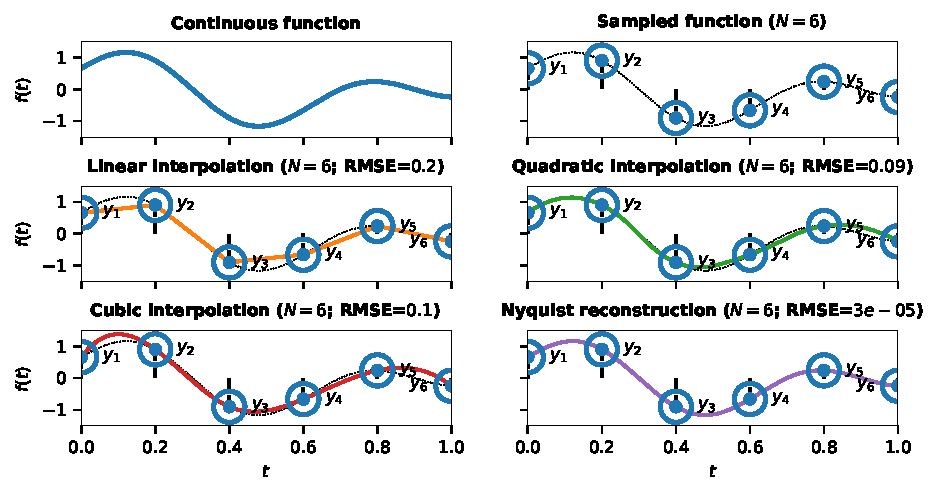
\includegraphics{media/fun_2_q6_small.pdf}
		\caption{Example 2: Bandlimit below $\SI{3}{\hertz}$}
	\end{subfigure}		
	\caption{Example illustrating sampling. A continuous function is sampled at $N = 6$ points (represented as a \enquote{lollipop} plot). We can use various interpolation techniques to reconstruct (\enquote{guess}) the values between individual sample points. In case the original function is bandlimited to a frequency below $N / {2T} = \SI{3}{\hertz}$ (as in \textbf{(b)}, but not \textbf{(a)}), the sample points uniquely define the function according to the Nyquist-Shannon sampling theorem.}
	\label{fig:sampling}
\end{figure}



\newpage

\paragraph{Guarantees for band-limited signals}
While the above restriction---namely, that we need infinitely many points to represent any infinitesimally small interval of a function---is true for general, mathematical functions, we have a much better guarantee regarding the required number of required for \enquote{physical}, i.e., band-limited, signals.

This guarantee is the Nyquist-Shannon sampling theorem, which connects the discrete, sampled world and continuous functions.
\begin{mdframed}
	\hfill\emph{(The Nyquist-Shannon Sampling Theorem)}\\
	If $f(t)$ contains no frequencies greater than $B$ then it is \emph{completely} determined by samples spaced $\Delta t = \frac{1}{2B}$ apart ($N = 2BT$ equally spaced samples for a time-slice $[0, T)$). There is a \emph{one-to-one mapping} between the samples $\vec x$ and the function $f(t)$.
\end{mdframed}
Note the emphasis on \enquote{one-to-one mapping}: if we have $N = 2BT$ equally spaced samples of a function with band-limit $B$, we can completely reconstruct the function without any losses. Of course, if we have access to the function, we can measure the sample points.

In summary, this means that there is hope that we can represent physical signals by storing just a few values. If we can guarantee that our function does not have any frequencies above $B$, we only need to store $N = 2BT$ samples; or, in other words we need to sample with a frequency of $f_\mathrm{s} = 2B$ (the \enquote{Nyquist Frequency}). So for a signal that is limited to \SI{5}{\hertz} we only need 10 samples per second to be able to perfectly reconstruct it. Conversely, there is no reason to store significantly more than $N$ samples---doing so would just be \enquote{wasting space}.

\Aside{\emph{The Nyquist-Shannon Sampling Theorem and Audio Signals.} There are some engineering related reasons for sampling slightly faster than the Nyquist frequency. For example, the absolute hearing threshold for (young) humans is about $B = \SI{20}{\kilo\hertz}$. Correspondingly, to record an audio signal meant for humans (i.e., music or speech recordings), we can do the following: (1) band-limit the original signal to \SI{20}{\kilo\hertz} in the capture device, (2) sample at $f_\mathrm{s} = \SI{40}{\kilo\hertz}$. This allows us to perfectly reconstruct the band-limited signal according to the Nyquist-Shannon sampling theorem. Since frequencies above \SI{20}{\kilo\hertz} are not audible, the result will appear to humans exactly as the original signal.

However, this only works if we can trust our capture device (i.e., the microphone and its amplifier circuit) to \emph{sharply} cut off all frequencies above $\SI{20}{\kilo\hertz}$. Unfortunately, such perfect filters are impossible to implement as an analogue device. Frequencies slightly above $B$ will still pass through, albeit being attenuated. This violates the pre-condition of the Nyquist-Shannon sampling theorem, leading to imperfect reconstructions (an effect known as \emph{aliasing}). Hence, it is better to sample faster than Nyquist, to give room for frequencies in the signal that are (slightly) above $B$.

This is why common sampling rates for audio signals are $\SI{44.1}{\kilo\hertz}$ (CD audio), and $\SI{48}{\kilo\hertz}$ (DVD audio). Much higher sampling of audio signals intended for human listening make no sense, except for intermediate signals (i.e., for sidestepping the imperfect analogue filter problem by sampling at a very high rate and applying a cheap and precise digital filter).}

\newpage

\vspace*{-0.75cm}
\Note{\emph{Online resources.} For more information on the Nyquist-Shannon sampling theorem in general, and its implications with respect to storing audio signals in particular, refer to this material by Chris Montgomery (author/co-author of the Ogg Vorbis and Opus codecs):
\begin{itemize}
	\item An excellent Video on the Nyquist Shannon sampling theorem, as well as quantisation: \href{https://xiph.org/video/vid2.shtml}{Xiph.org Digital Show and Tell, Episode 2}.
	\item An article on \enquote{\href{https://people.xiph.org/~xiphmont/demo/neil-young.html}{24 bit / 192 kHz Music Downloads
and why they make no sense}}; this may seem tangential but explains the above in much more detail.
\end{itemize}}

\Note{\emph{Algorithm for the \enquote{Nyquist Reconstruction} of Functions.}
The Nyquist-Shannon sampling theorem tells us that it is possible to perfectly reconstruct a function with band limit $B$ as long as we have $N = 2BT$ equally spaced sample points. But how do we compute this reconstruction for discrete signals in practice? Put differently, how do we convert $N$ sample points ${x'}_0, \ldots, {x'}_N$ into a densely sampled signal $x_0, \ldots, x_M$ with $M \geq N$. The answer is to use the Fourier transformation of the sample points.

First consider the reverse direction. We're given a signal with band limit $B$ and $M \geq N$ equally spaced sample points $x_0, \ldots, x_M$. We can then compute the corresponding Fourier coefficients $\omega_{-M/2}, \ldots, \omega_{0}, \ldots \omega_{M/2}$. If a function is band-limited with band-width $B$, this means that only the $N = 2BT$ frequency coefficients $\omega_{-BT}, \ldots, \omega_0, \ldots, \omega_{BT}$ are nonzero. Discarding the zero-coefficients and converting the remaining $N$ frequency coefficients back to the time-domain results in $2BT$ equally spaced sample points in the time domain, ${x'}_0, \ldots, {x'}_N$.

Hence, if we want to convert ${x'}_0, \ldots, {x'}_N$ to $x_0, \ldots, x_M$ with $M \geq N$, we perform the above steps in reverse: we convert ${x'}_0, \ldots, {x'}_N$ to the Fourier domain, pad with leading and trailing zeros so we have $M$ frequency coefficients, and convert to the time-domain.

In practice, there are more efficient ways to do this (i.e., interlacing the signal with zeros, applying the right FIR/IIR filter and selecting $M$ samples). This process is also known as \emph{sampling rate conversion}.}

\subsection{Basis Functions}

Another popular way of representing functions as vectors is to express them in terms of a linear combination of a set of basis functions. Let $\phi_1, \ldots, \phi_q$ be functions $\mathbb{X} \subset \mathbb{R} \longrightarrow \mathbb{R}$. In case we chose these basis functions well, we can approximate a wide range of $f$ with a low error over some interval $\mathbb{X}$ by linearly combining the basis functions:
\begin{align}
	f(t) \approx \hat f(t) = \sum_{i = 1}^q x_i \phi_i(t) \,.
	\label{eqn:eval_f}
\end{align}
The vector $\vec x = (x_1, \ldots, x_q)$ now encodes the function.

A different way of reading the above equation is that we can evaluate the encoded function $\hat f(t)$ at a point $t$ by computing a dot product $\langle \vec a, \vec x \rangle$, where $a_i = \phi_i(t)$. Put differently, if we know the point $t$ at which we want to evaluate $\hat f(t)$, we can pre-compute a $\vec a$ to decode the represented function at this point.

\paragraph{Computing the vector coefficient of $\vec x$ for orthonormal function bases.}
Given the above, how do we compute the $\vec x$ that encodes a function $f$. To a degree, this depends on the choice of the basis functions. In the special case of an \emph{orthonormal} function basis, that is
\begin{align*}
	\langle \phi_i, \phi_j \rangle = \int_{\mathbb{X}} \phi_i(t) \phi_j(t) \, \mathrm{d}t = \begin{cases}
		1 & \text{if } i = j \,,\\
		0 & \text{otherwise} \,,
	\end{cases}
\end{align*}
then each coefficient of $\vec x = (x_1, \ldots, x_q)$ is just given as
\begin{align}
	x_i &= \langle \phi_i, f \rangle = \int_{\mathbb{X}} f(t) \phi_i(t) \, \mathrm{d}t \,.
	\label{eqn:ortho_transform}
\end{align}
\vspace*{-0.4cm}

\Note{\emph{Relationship between sampling and basis functions.} Sampling can be seen as a special case of using basis functions. In particular, if we choose a set of Dirac-$\delta$ functions $\phi_i(t) = \delta(t - \Delta t i)$ as basis functions, then \cref{eqn:ortho_transform} will exactly \enquote{read out} the function values at $\Delta t i$. This is just a consequence of the definition of the Dirac-$\delta$ (see the notes for lecture two and four); it holds
\begin{align*}
	x_i = \int_{\mathbb{X}} f(t) \delta(t - \Delta t i) \, \mathrm{d}t = f(\Delta ti) \,.
\end{align*}}

\Note{\emph{Basis functions and the Fourier/Laplace transformation.} Notice that this is very similar to the equation underlying the Fourier or Laplace transformations that we saw earlier in the course. This is exactly because these transformations can be described in terms of an orthonormal function basis.

The same equation---i.e., computing the dot-product between the value that should be represented and the basis---is also used when representing a vector in terms of an orthonormal vector basis. In a sense, we are just computing \enquote{how similar} the represented value is to each basis vector/function, giving us the vector coefficients with respect to the new basis.}

\paragraph{Computing the vector coefficients of $\vec x$ in the general case.}
In the general case, we can compute the coefficients of $\vec x$ by sampling and solving a least squares problem
\begin{align*}
	\vec x = \arg\min_{\vec x} \sum_{k = 1}^N \sum_{i = 1}^q \big( f(t_k) - x_i \phi_i(t_k) \big)^2 \,,
\end{align*}
where $t_1, \ldots, t_N$ are a set of $N$ sample points. Note that this is exactly the optimization problem we solve when computing population decoders $\mat D$. This is not a coincidence; the tuning curves in a neuron ensemble form a set of basis functions.

\paragraph{Popular basis functions} So what are some popular basis functions that people use to represent functions over time? As mentioned above, we have already seen the Fourier and Laplace transformation, which---at least in their discrete versions---can be thought of as a basis transformation.

\begin{figure}[p]
	\centering
	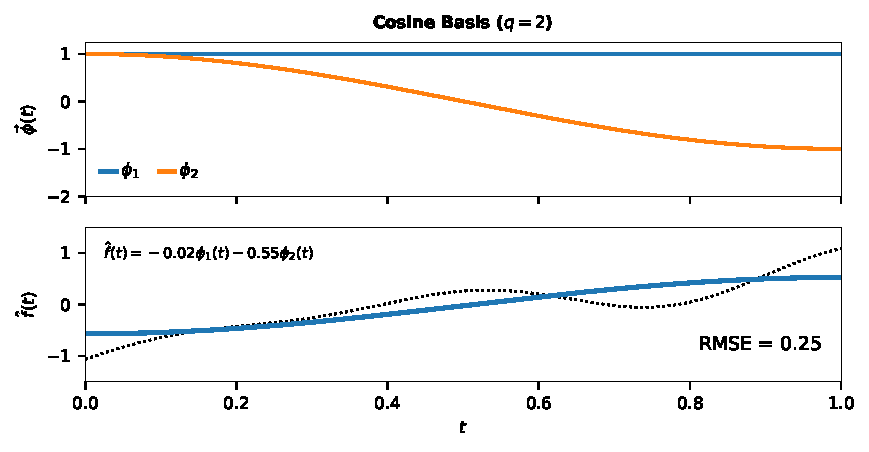
\includegraphics[scale=0.95]{media/cosine_q2.pdf}
	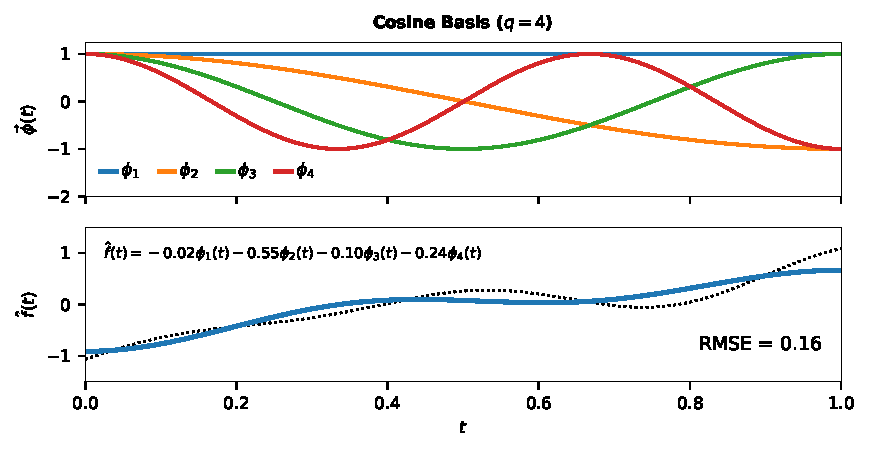
\includegraphics[scale=0.95]{media/cosine_q4.pdf}
	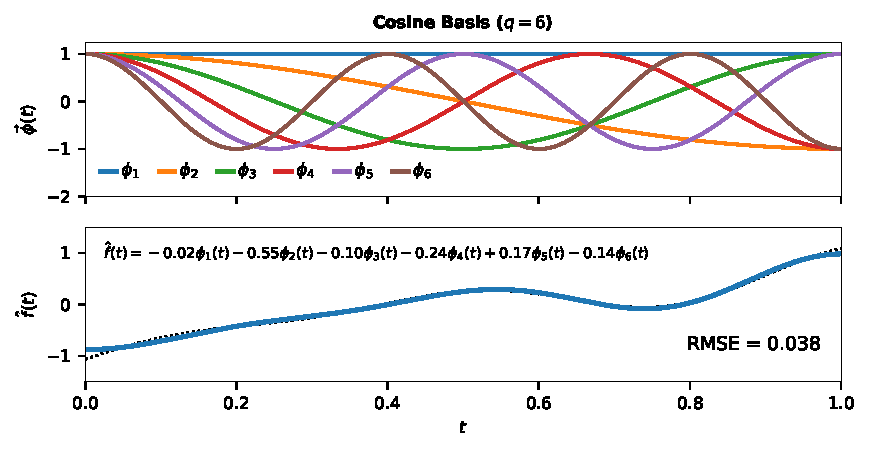
\includegraphics[scale=0.95]{media/cosine_q6.pdf}
	\caption{Representing a function (dotted line in the bottom plots) with a variable number $q$ of cosine basis functions over the interval $\mathbb{X} = [0, 1]$. The error goes to zero as $q$ increases.}
	\label{fig:cosine}
\end{figure}
Another popular (orthonormal) basis is the discrete cosine basis and the associated discrete cosine transformation (DCT, cf.~\cref{fig:cosine}). There are multiple versions of the DCT basis. One particular version is given as
\begin{align*}
	\phi_i(t) &= \cos\big( (i - 1) \pi t \big) \quad \text{for } t \in \mathbb{X} = [0, 1] \,. && \textit{(Discrete Cosine Basis)}
\end{align*}

\begin{figure}[p]
	\centering
	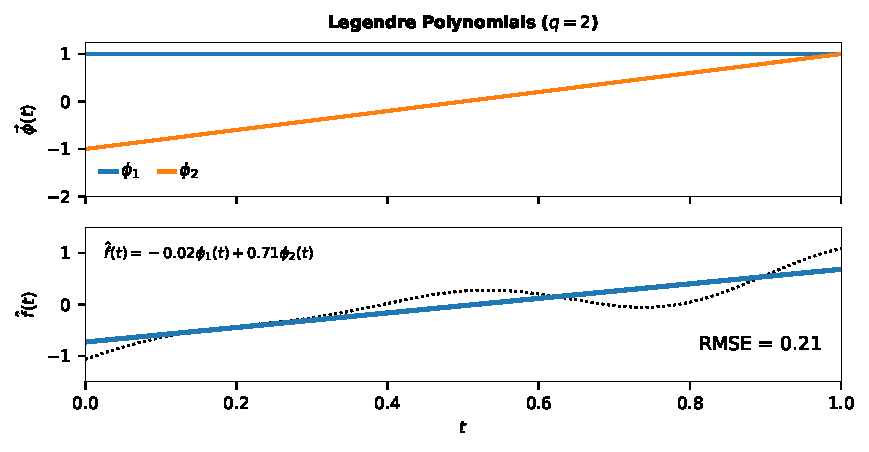
\includegraphics[scale=0.95]{media/legendre_q2.pdf}
	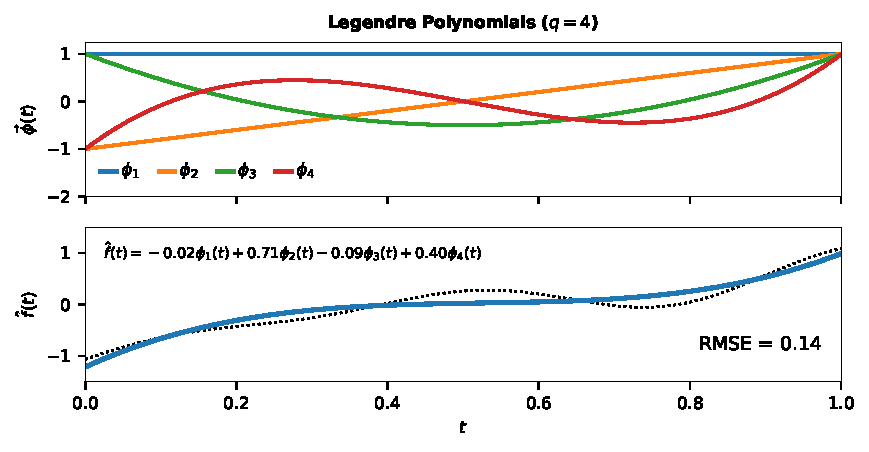
\includegraphics[scale=0.95]{media/legendre_q4.pdf}
	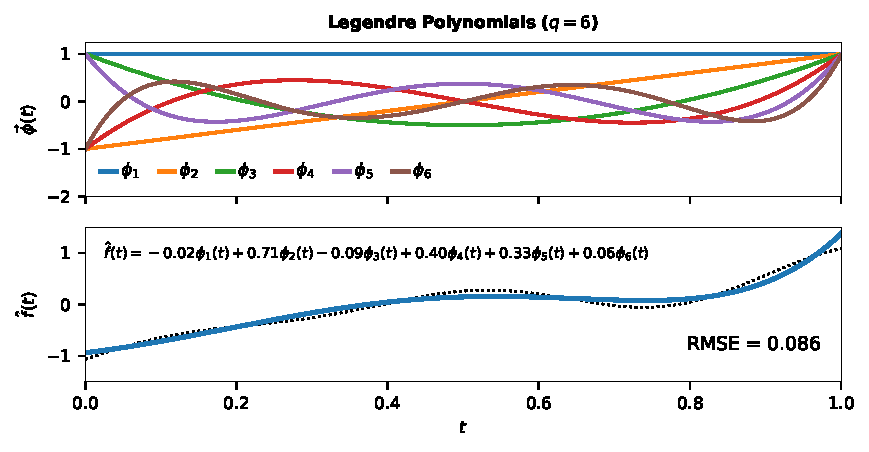
\includegraphics[scale=0.95]{media/legendre_q6.pdf}
	\caption{Representing a function (dotted line in the bottom plots) with a variable number $q$ of shifted Legendre polynomials over the interval $\mathbb{X} = [0, 1]$. The error goes to zero as $q$ increases.}
	\label{fig:legendre}
\end{figure}
Another popular set of basis functions (which are orthogonal, but not ortho\emph{normal}) is the Legendre basis (\cref{fig:legendre}). This is a so called \enquote{polynomial} basis, which means that the $i$th basis function is a polynomial of order $i$ when counting from zero. The (shifted) Legendre basis is given as
\begin{align}
	\phi_i(t) = \tilde P_i(t) = (-1)^{i} \sum_{k=0}^{i} \binom{i}{k} \binom{i + k}{k} (-t)^{k} \quad \text{for } t \in \mathbb{X} = [0, 1]\,. && \textit{(Shifted Legendre Basis)}
	\label{eqn:legendre}
\end{align}

These are shifted in the sense that they are symmetric over [0,1] rather than [-1,1].

\section{Representing the Past: The Delay Network}

We discussed two techniques for representing functions as vectors. The first technique, sampling, has taught us that there are mathematical guarantees regarding the representation of bandlimited functions. As long as our function $f$ is band-limited, we know that we can perfectly represent an interval $\mathbb{X}$ as a finite number of coefficients $\vec x = (x_1, \ldots, x_N)$. The higher the maximum frequency $B$ in the signal, the more coefficients are required to represent it. This relationship is less clear for the second technique we discussed, basis functions, but in practice, since many function space representations map higher frequencies onto basis functions $\phi_i(t)$ higher indices $i$, similar constraints hold here as well.

However, it is still unclear how to \emph{encode} a function $f$ in a neural ensemble as a vector $\vec x$. If we were given a set of samples $x_1, \ldots, x_N$, we could either use those samples directly as our function representation, or alternatively, if we wanted to represent these points with respect to an orthonormal/orthogonal function basis, we can use a linear transformation to transform the samples into the corresponding function space.

This still does not answer the question of where these samples come from. In particular, given the goal that we want to represent a sliding window over the past, we need a technique to somehow readjust our representation $\vec x$ in each time step.

\subsection{Implementing Delays as a Dynamical System}

In order to solve this problem, let's start fresh and think about this from a different perspective---we will come back to what we discussed in the previous section at the end. 

One way of remembering a window of time $[t - \theta, t]$ is to implement a delay of $\theta$ seconds as a dynamical system. This may sound a little counter intuitive---how does implementing a \emph{delay} help us to remember all the information within a time-window $[t - \theta, t]$? Actually, thinking about this a little more, when building a dynamical system that implements a delay, there is no way around remembering the entire time-window. There \emph{has} to be information about all the time points in the interval $[t - \theta, t]$ in the system, because---as time $t$ progresses---any point within that interval will eventually be located at $t - \theta$.


\begin{itemize}
	\item \textbf{Motivation:} Implement a perfect delay of a time $\theta$ in the Neural Engineering Framework.
	\item This can be seen as a dynamical system. In the Laplace Domain, a perfect delay is $e^{-s\theta}$.
	\item Use Padé approximants up to a degree $q$ to compute an LTI system approximating $e^{-s\theta}$. This system has a one-dimensional input $u(t)$ and an internal state $\vec x(t)$ of dimension $q$:
	\begin{align}
		\vec x(t) &= \mat A \vec x(t) + \mat B u(t) \\
	    \theta \mat{A} &= a_{ij} \in \mathbb{R}^{q \times q} \,, & \kern-0.5em a_{ij} &= \begin{cases}
		(2i + 1)(-1) & \kern-0.5em i < j \,,\\
		(2i + 1)(-1)^{i - j + 1} & \kern-0.5em i \geq j \,,
		\end{cases}\\
		\theta \mat{B} &= b_i \in \mathbb{R}^{q} \,, & \kern-0.5em b_i &= (2i + 1)(-1)^i \,.
		\label{eqn:delay_network_lti}
	\end{align}
	\item We can implement this LTI system as a neural ensemble using the transformation
	\begin{align*}
		\mat A' &= \tau \mat A + \mat I \,,\\
		\mat B' &= \tau \mat B \,.
	\end{align*}
	\item The state $\vec x \in \mathbb{R}^q$ represents more information than just the input $\theta$ seconds ago. It represents the state at every point in time up to $\theta$ seconds.
	\item In fact, $\vec x$ represents the function $f_{[t - \theta, t]}\left(\frac{\theta'}{\theta}\right) \approx u\left(t' - \theta' \right)$ in the Legendre basis
	\begin{align*}
		u\left(t' - \theta' \right) \approx f_{[t - \theta, t]}\left(\frac{\theta'}{\theta}\right) &= \sum_{i=1}^q \tilde P_i \left( \frac{\theta'}{\theta} \right) x_i(t) \,.
	\end{align*}
	\item When representing $\vec x$ in neurons, we can not only decode delays but any function using information from the past $\theta$ seconds.
	\item This network implements an optimal recurrent neural network remembering a slice of the past, as a so called \enquote{reservoir}.
\end{itemize}

\subsection{Example: Implementing the Delay Network in Nengo}

The above may seem a little abstract---correspondingly, we use this section to describe how to actually implement the Delay Network in Python.

\paragraph{Step 1: Computing the matrices $\mat A$, $\mat B$.}
First, we need to compute $\mat A$ and $\mat B$ as defined in \cref{eqn:delay_network_lti}. These matrices depend on two paramters: $q$, the number of state dimensions, and $\theta$, the length of the time window. The following code has been adapted from Aaron Voelker's \texttt{nengolib}\footnote{\url{https://github.com/arvoelke/nengolib}} library and computes these matrices in a few lines of Python.
\cprotect\Python{\begin{lstlisting}[morekeywords={with,as}]
def make_delay_network(q, theta):
    Q = np.arange(q, dtype=np.float64)
    R = (2 * Q + 1)[:, None] / theta
    j, i = np.meshgrid(Q, Q)
    A = np.where(i < j, -1, (-1.)**(i - j + 1)) * R
    B = (-1.)**Q[:, None] * R
    return A, B
\end{lstlisting}}

\paragraph{Step 2: Computing the equivalent neural LTI system matrices.}
We can then turn these matrices into the feedback and input matrices $\mat A'$ and $\mat B'$ for a recurrently connected neural ensemble as discussed in the previous lecture. To this end, we use a generic function that takes $\tau$, $\mat A$, and $\mat B$ and outputs the adapted matrices $\mat A'$ and $\mat B'$.
\cprotect\Python{\begin{lstlisting}[morekeywords={with,as}]
def make_nef_lti(tau, A, B):
    Ap = tau * A + np.eye(A.shape[0])
    Bp = tau * B
    return Ap, Bp
\end{lstlisting}}

\paragraph{Step 3: Computing a Delay Decoder.}
In order to decode a delay $\theta'$ from the function representation $\vec x$ according to \cref{eqn:eval_f}, we need to evaluate the Legendre polynomials at $\frac{\theta'}{\theta}$. Numpy implements Legendre polynomials in its \texttt{np.polynomial} module, so we do not have to worry about writing code for \cref{eqn:legendre} ourselves.
\cprotect\Python{\begin{lstlisting}[morekeywords={with,as}]
def make_delay_decoder(q, thetap, theta=1.0):
    ts = np.array(thetap / theta) # Compute the ratio between thetap and theta
    return np.array([np.atleast_1d(
        # Evaluate the Legendre polynomial of order "i" shifted to [0, 1] at "ts"
        np.polynomial.Legendre([0] * i + [1], [0, 1])(ts)) for i in range(q)])
\end{lstlisting}}

\paragraph{Step 4: Building the network.}
Using Nengo, we use the system matrices $\mat A'$ and $\mat B'$ to implement the recurrent neural network.
\cprotect\Python{\begin{lstlisting}[morekeywords={with,as}]
q, theta, tau = 6, 0.5, 0.1
Ap, Bp = make_nef_lti(tau, *make_delay_network(q, theta)) # 
dec_250 = make_delay_decoder(q, 0.25, theta) # 250ms delay
with nengo.Network() as model:
    nd_in = nengo.Node(nengo.processes.WhiteSignal(
        high=2.0, period=10.0, rms=0.5))
    nd_out = nengo.Node(size_in=1)
    ens_x = nengo.Ensemble(
        n_neurons=500, dimensions=q,
        intercepts=nengo.dists.CosineSimilarity(q + 2))
    nengo.Connection(nd_in, ens_x, transform=Bp, synapse=tau)
    nengo.Connection(ens_x, ens_x, transform=Ap, synapse=tau)
    nengo.Connection(ens_x, nd_out, transform=dec_250.T)
\end{lstlisting}}
When executing this network, \texttt{ens\_x} represents the $q$-dimensional state vector $\vec x$ that encodes the past $\theta$ seconds in the Legendre function space, i.e., $f_{[t - \theta, t]}$ in the notation used above. We could for example use the PES learning rule to learn a function that depends on  $f_{[t - \theta, t]}$. In the above example, we just chose to compute a delay---the output node \texttt{nd\_out} will contain the input delayed by \SI{250}{\milli\second}.
\Note{\emph{Using the cosine similarity distribution as intercept distribution.}
You may have noticed the line \texttt{intercepts=nengo.dists.CosineSimilarity(q + 2)} in the above code. This selects the tuning curve intercepts according to the distribution of the cosine similarity between random vectors in $q + 2$ dimensions. Doing this is useful when building high-dimensional neural ensembles---without adapting the intercepts, many neurons end up not firing at all over large ranges of the represented space. With the adapted intercepts, the input current distribution stays approximately constant. See \href{https://github.com/tcstewar/testing_notebooks/blob/master/Intercept\%20Distribution\%20.ipynb}{this Jupyter Notebook} by Terrence C.~Stewart and this tech report \cite{voelker2017efficiently} for more details.
}

\printbibliography

\end{document}

